%%%%%%%%%%%%%%%%%%%%%%%%%%%%%%%%%%%%%%%%%%%%%%%%%%%%%%%%%%%%%%%%%%%%%%%%%%%%%%%%
%2345678901234567890123456789012345678901234567890123456789012345678901234567890
%        1         2         3         4         5         6         7         8

\documentclass[letterpaper, 12 pt, conference]{ieeeconf}  % Comment this line out
                                                          % if you need a4paper
%\documentclass[a4paper, 10pt, conference]{ieeeconf}      % Use this line for a4
                                                          % paper

\IEEEoverridecommandlockouts                              % This command is only
                                                          % needed if you want to
                                                          % use the \thanks command
\overrideIEEEmargins
% See the \addtolength command later in the file to balance the column lengths
% on the last page of the document



% The following packages can be found on http:\\www.ctan.org
\usepackage{graphicx} % for pdf, bitmapped graphics files
\usepackage{bm}
\usepackage{listings}
\usepackage{graphicx}

\usepackage{biblatex}
\addbibresource{bibliography.bib}

\newcommand{\uvec}[1]{\boldsymbol{\hat{\textbf{#1}}}}
%\usepackage{epsfig} % for postscript graphics files
%\usepackage{mathptmx} % assumes new font selection scheme installed
%\usepackage{times} % assumes new font selection scheme installed
%\usepackage{amsmath} % assumes amsmath package installed
%\usepackage{amssymb}  % assumes amsmath package installed

\title{\LARGE \bf
Modeling Geomagnetic Induced Currents Using Computer-Based
Simulations
}

%\author{ \parbox{3 in}{\centering Huibert Kwakernaak*
%         \thanks{*Use the $\backslash$thanks command to put information here}\\
%         Faculty of Electrical Engineering, Mathematics and Computer Science\\
%         University of Twente\\
%         7500 AE Enschede, The Netherlands\\
%         {\tt\small h.kwakernaak@autsubmit.com}}
%         \hspace*{ 0.5 in}
%         \parbox{3 in}{ \centering Pradeep Misra**
%         \thanks{**The footnote marks may be inserted manually}\\
%        Department of Electrical Engineering \\
%         Wright State University\\
%         Dayton, OH 45435, USA\\
%         {\tt\small pmisra@cs.wright.edu}}
%}

\author{Nikhil Nayak}




\begin{document}



\maketitle
\thispagestyle{empty}
\pagestyle{empty}


%%%%%%%%%%%%%%%%%%%%%%%%%%%%%%%%%%%%%%%%%%%%%%%%%%%%%%%%%%%%%%%%%%%%%%%%%%%%%%%%
\begin{abstract}

Geomagnetic disturbances (GMDs) are caused when the sun emits a coronal mass ejection (CME), a large expulsion of magnetic fields. When the CME collides with Earth's magnetic field, the collision generates currents that create Geomagnetically Induced Currents (GICs). GICs can disturb electrical systems in the affected areas. The March 1989 Quebec incident displays an example of the effects of GMDs, causing a nine-hour power outage. \cite{8859181} works to derive the equations necessary to model GMDs. However, computer-based implementations require specific methods for accurate modeling. This project researches the development of a GMD model on a computer using the Julia programming language. 

\end{abstract}


%%%%%%%%%%%%%%%%%%%%%%%%%%%%%%%%%%%%%%%%%%%%%%%%%%%%%%%%%%%%%%%%%%%%%%%%%%%%%%%%
\section{INTRODUCTION}

Geomagnetic disturbances, also referred to as "geomagnetic storms", are caused by a transfer of energy of charged particles from the sun to the space surrounding Earth. GMDs are especially dangerous due to the variability of their effects. While the presence of GMDs can be predicted, the effect and magnitude cannot be. The currents produced by the GMDs create electric fields at the Earth's surface. The currents can flow into conducting networks such as power grids or telephone networks, damaging equipment and devices in these networks. Based on the scale of the GMD, the effect can be as large as city-wide blackouts. The process to help mitigate the effects of GMDs is made up of three parts. First, data must be collected for the required area. Second, the collected data must be processed by a transfer function model. Lastly, the data from the model can be used to determine the necessary currents to properly power the affected networks. This paper focuses on the implementation of the second stage, the transfer function model. For the model, the 5 layer Quebec model developed in \cite{8859181} is used.


\section{Implementation}
The implementation of the 5 layer Quebec model is done in the Julia programming language, using \verb|Trapz| for trapezoidal integration, \verb|PyPlot| for plots, and \verb|FFTW| for Fourier transforms.

\subsection{Synthetic Dataset}
First, a synthetic dataset was created for testing. The synthetic field variation was calculated using the sum of 7 sinusoidal functions. The code for the data was implemented using the following code:
\begin{lstlisting}
A =   [200, 90, 30, 17, 8, 3.5, 1]
Phi = [10, 20, 30, 40, 50, 60, 70]

f = [0.00009259, 0.00020833, 
0.00047619, 0.00111111, 0.00238095, 
0.00555555, 0.025]

function B(t) # Equation (20)
  y = 0
  for i in 1:7
    y += A[i] * sin(
      2 * pi * f[i] * t 
	  + (pi / 180 * Phi[i])
	)
	end
  return y
end
\end{lstlisting}

Using the \verb|B| function, the synthetic variation can be found for any second \verb|t|. In Julia, this can be implemented simply using the vectorization operators like so:

\begin{lstlisting}
timestep = 1
X = 1:timestep:86400
Y = B.(X)
\end{lstlisting}

\begin{figure}
    \centering
    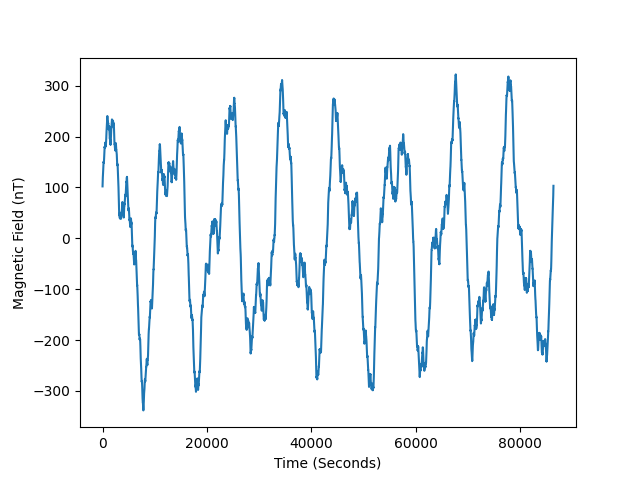
\includegraphics[width=\columnwidth]{Figure_1.png}
    \caption{Synthetic Field Variation Graph}
    \label{fig:my_label}
\end{figure}

\begin{figure}
    \centering
    \includegraphics[width=\columnwidth]{Figure_2.png}
    \caption{Discrete Fourier Transformer of B(t) - A correct implementation should include 7 lines on each side of x=0, representing the 7 sine functions in B(t)}
    \label{fig:my_label}
\end{figure}



\subsection{Discretization}
\label{discretization}
Because this implementation is done on a computer with a finite amount of memory, processing power, etc., the continuous function cannot be represented on a computer and must be discretized using a Fourier transform. The following code is used to discretize the \verb|B| function using the FFTW library:
\begin{lstlisting}
f = fft(Y)
\end{lstlisting}

Additionally, the horizontal geoelectric field, E(f) is calculated as the convolution of B and K, defined in Julia like so:
    
\begin{lstlisting}
function K(f)
    mu = pi * 4e-6
    sigma = 1000
    i = 1im
    return sqrt(
        (i * 2 * pi * f) /
        (mu * sigma)
    )
end
\end{lstlisting}
    
and the convolution of the signals is calculated like so:
    
\begin{lstlisting}
freq = fftfreq(length(Y), timestep)
conv = K.(freq) .* f
\end{lstlisting}

This code creates and processes the synthetic field variation data. Next, a model needs to be developed to model the input data.

\subsection{5 Layer Quebec Model}
The model used in this paper is the 5 layer Quebec model used to model Earth conductivity in \cite{8859181}. The model is represented by 5 equations, each of which use the previous equation. This is implemented in Julia using recursion with the base case being the topmost layer. Each layer has distinct thicknesses and relativities. The thicknesses and relatives are as followed:

\vspace{1cm}
{\begin{tabular}{|c|c|c|}
\hline
Layer & Thickness (Km) & Resistivity ($\Omega$ m) \\
\hline
1 & 15 & 1/20000 \\
\hline
2 & 10 & 1/200 \\
\hline
3 & 125 & 1/1000 \\
\hline
4 & 200 & 1/100 \\
\hline
5 &  & 1/3 \\
\hline
\end{tabular}}
Layer 5 is not defined using the table and recursive function. Instead, layer 5 is the base case. The base case and recursive function are defined as so:

\begin{lstlisting}[linewidth= \columnwidth]
thickness = [1/20000, 1/200, 1/1000,
    1/100, 1/3] * 1e3
resistivity = [20000, 200, 1000, 100]

N = 5 # number of layers in the model
mu = pi * 4e-6
i = 1im
\end{lstlisting}
- Code continuted on next page -
\begin{lstlisting}


function K_Base(f)
    return sqrt((i * 2 * pi * f) /
    (mu * thickness[N]))
end

function k(n, f)
    return sqrt(i * 2 * pi * f 
    * mu * thickness[n])
end

function eta(n, f)
    return i * 2 * pi * f 
    / k(n, f)
end

function eExpr(n, f)
    return e ^ (-2 * k(n, f)
    * resistivity[n])
end

function K(n, f) # Equation 19
    if n == N
            return K_Base(f)
    end

    K_NPrev = K(n+1, f)
    e = eExpr(n, f)
    
    num = K_NPrev * (1 + e) 
    + eta(n, f) * (1 - e)
    
    den = K_NPrev * (1 - e) 
    + eta(n, f) * (1 + e)
    
    return eta(n, f) * num / den
end

function K(f)
    return K(1, f)
end
    \end{lstlisting}

The function K (not to be confused with the K in \ref{discretization}) is the complete implementation of the 5-layer Quebec model.

\vspace{1cm}

\section{Benchmark}
To evaluate the accuracy of the computer implementation, it must be compared to the results from the original paper. Table 4 in \cite{8859181} shows the values calculated by the transfer function. This can be compared to the results calculated using the computer implementation above. 


\begin{figure}
    
    \centering
    
    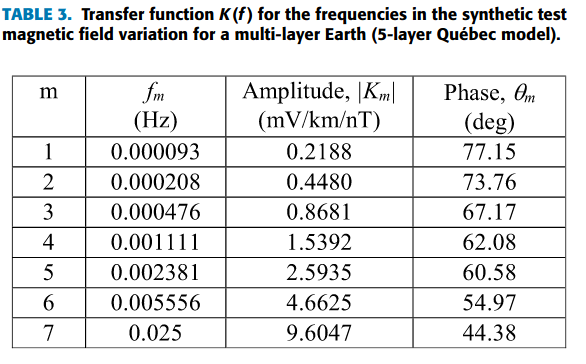
\includegraphics[width=\columnwidth]{Figure_3.png}
		    
		    %\includegraphics[width=\columnwidth]{Latex/Figure_2.png}
		    
		  {\begin{tabular}{|c|c|c|c|}
        \hline
        m & $f_m$ & Amplitude & Phase \\
        \hline
        1 & 0.000093 & 0.219701 & 77.139393 \\
        \hline
        2 & 0.000208 & 0.447422 & 73.771382 \\
        \hline
        3 & 0.000476 & 0.867800 & 67.172638 \\
        \hline
        4 & 0.001111 & 1.539096 & 62.080986 \\
        \hline
        5 & 0.002381 & 2.593561 & 60.575656 \\
        \hline
        6 & 0.005556 & 4.662704 & 54.969143 \\
        \hline
        7 & 0.025 & 9.604690 & 44.381495 \\
        \hline
    \end{tabular}}
		    

		\caption{Transfer function results from \cite{8859181}}
		\caption{Results from function implemented above}
	\end{figure}

Based on the tables, the computer simulation is very accurate; any inaccuracy is most likely due to the inaccuracy of calculations, constants, or the FFTW library. 
     
\vspace{6cm}

\section{Real World Application}
The 5 layer model implemented above can be used with real data rather than a simulated dataset. In this paper, a Fort Simpson, Canada dataset is used. For each value in the time-series data, the value was used as input to the transfer function \verb|K|. This can be vectorized in Julia like so:
	
\begin{lstlisting}
Y = K.(X)
\end{lstlisting}
	
The lines in Fig. 5 show both the input from the Fort Simpson data as well as the transfer function data.

\begin{figure}
    \label{fig:fsim}
	   \begin{center}
	        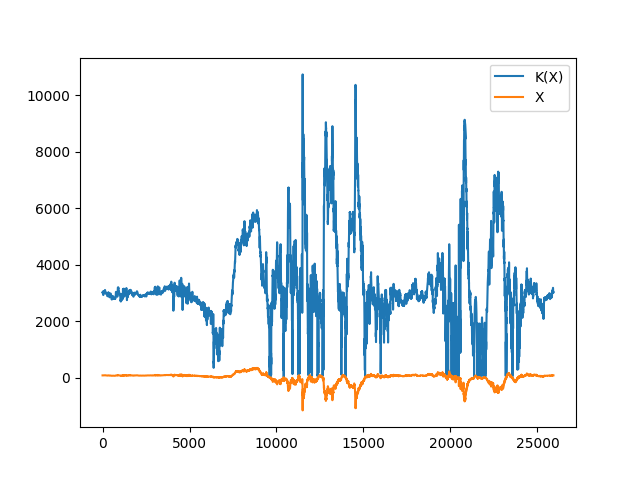
\includegraphics[width=\columnwidth]{fsim.png}
	       \caption{Sensor data and transfer function data from Fort Simpson dataset}
	   \end{center}
	
	\end{figure}  


    

\nocite{*}
\printbibliography




\end{document}
